\documentclass{beamer}

\usepackage{beamerthemesplit}
\usetheme{Singapore} %Copenhagen}
%\usecolortheme{whale}

%\usepackage[T2A]{fontenc}
%\usepackage[utf8]{inputenc}
%\usepackage[russian]{babel}

\usepackage[main=russian,english]{babel}   %% загружает пакет многоязыковой вёрстки
\usepackage{fontspec}      %% подготавливает загрузку шрифтов Open Type, True Type и др.
\defaultfontfeatures{Ligatures={TeX},Renderer=Basic}  %% свойства шрифтов по умолчанию
\setmainfont{Times New Roman} %% задаёт основной шрифт документа
%\usefonttheme{professionalfonts}% SOLUTION
\usefonttheme{serif}

\usepackage{hyperref}
\usepackage{textcomp}
\usepackage{amssymb,amsmath}
%\usepackage{animate}
%\usepackage{longtable}
\usepackage{xcolor}

%\usepackage{pgffor}
\usepackage{enumitem}


\newcounter{N}

%% Форматирование окружения itemize
%\usepackage{ragged2e}
%\let\olditem\item
%\renewcommand\item{\olditem\justifying}


\newcommand{\argxi}{(\xi^1,\xi^2,\xi^3)}
\newcommand{\argx}{(x^1,x^2,x^3)}

\newcommand{\argxbarn}{(\bar{x}^1,\bar{x}^2,\ldots, \bar{x}^n)}
\newcommand{\argxn}{(x^1, x^2,\ldots, x^n)}

\newcommand{\argtxi}{(t, \xi^1,\xi^2,\xi^3)}
\newcommand{\argtoxi}{(t_0, \xi^1,\xi^2,\xi^3)}

\newcommand{\argtx}{(t, x^1,x^2,x^3)}
\newcommand{\argtox}{(t_0, x^1,x^2,x^3)}

\newcommand{\pd}[2]{\frac{\partial #1}{\partial #2}}
\newcommand{\pdk}[2]{\frac{\partial^2 #1}{\partial {#2}^2}}

\title[]{Cилы, действующие на сплошную среду, тензор напряжений}

\author[]{ {\em Верещагин Антон Сергеевич}
\\
канд. физ.-мат. наук, старший преподаватель\\
\bigskip
Кафедра аэрофизики и газовой динамики ФФ НГУ}

\usebackgroundtemplate{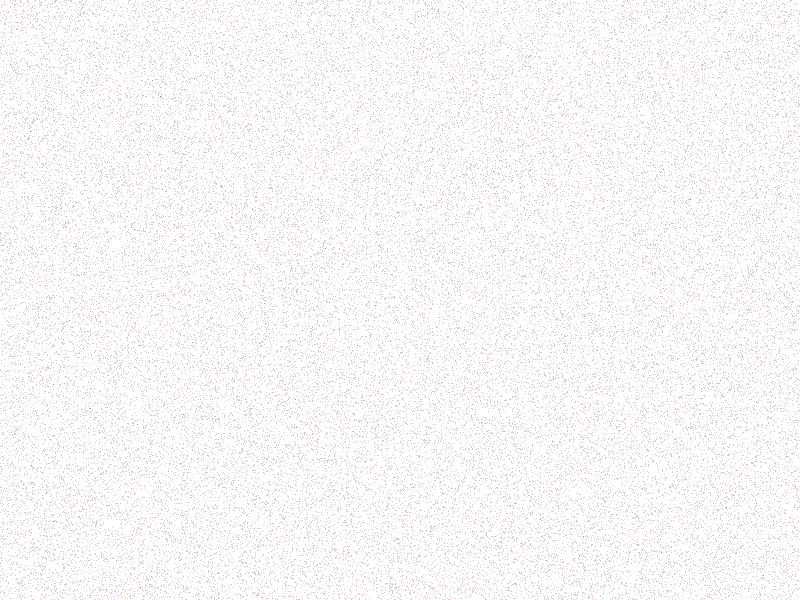
\includegraphics[width=\paperwidth]{../img/background.png}}

\begin{document}
	
\frame{\titlepage}


\frame{
	\frametitle{Аннотация}
	\parbox{\textwidth}{
		Объемные и массовые силы. Поверхностные силы. Тензор напряжения Коши. Разложение напряжения на составляющие. Главные напряжения и оси тензора напряжения. 
	}
}

\frame{
	\frametitle{ Объемные и массовые силы }
	
	\begin{exampleblock}{Определение }
		\parbox{\textwidth}{
			Силы, действующие на каждый элемент объема $d\omega$ независимо от того, существуют ли рядом с объемом $d\omega$ другие частицы или нет, называются  \alert{объемными}. 	Если такие силы отнесены к единице массы, то они называются \alert{массовыми}.
		}
	\end{exampleblock}\pause

	\begin{exampleblock}{Пример}
		\parbox{\textwidth}{
		Объемная сила, действующая на частицу среды в поле силы тяжести, определяется соотношением
		\[
		d\vec{F} = \rho \vec{g} d\omega,
		\]
		где $\rho$ -- плотность жидкой частицы, $\vec{g}$ -- вектор ускорения свободного падения.
		}
	\end{exampleblock}
}

\frame{
	\frametitle{ Поверхностные силы }
	
	\begin{columns}
		\begin{column}{0.35\textwidth}
			\parbox{\textwidth}{
				\centering
				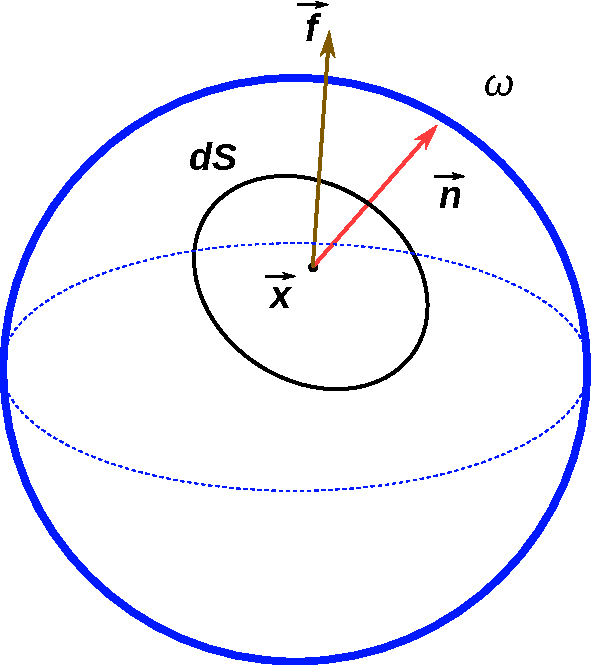
\includegraphics[width=\textwidth]{../img/sigma_def.pdf}
				
				\medskip	
				\scriptsize
				\parbox{\textwidth}{
				Выделенный объем сплошной среды $\omega$, с фиксированной точкой $\vec{x}$ внутри него и элементарной площадкой $dS$ с единичной нормалью $\vec{n}$		

				}

			}
		\end{column}
		\begin{column}{0.65\textwidth}
			\begin{exampleblock}{Определение }
				\parbox{\textwidth}{
					\alert{Напряжением поверхностной силы} $\vec{f}$ называется величина силы, отнесенная к элементарной площадке $dS$ с единичной нормалью $\vec{n}$, возникающая в результате взаимодействия частей среды с разных сторон от элементарной площадки в малой окрестности точки $\vec{x}$. 
				}
			\end{exampleblock}
		

		\end{column}
	\end{columns}
}

\frame{
	\frametitle{ Поверхностные силы  }
		\begin{columns}
		\begin{column}{0.35\textwidth}
			\parbox{\textwidth}{
				\centering
				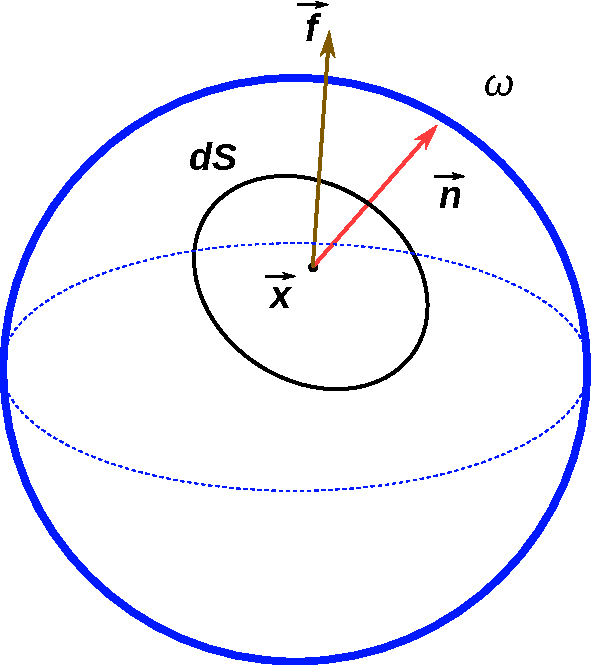
\includegraphics[width=\textwidth]{../img/sigma_def.pdf}
				
				\medskip	
				\scriptsize
				\parbox{\textwidth}{
					Выделенный объем сплошной среды $\omega$, с фиксированной точкой $\vec{x}$ внутри него и элементарной площадкой $dS$ с единичной нормалью $\vec{n}$					
				}
				
			}
		\end{column}
		\begin{column}{0.65\textwidth}
			
			\begin{exampleblock}{Замечания}
				\parbox{\textwidth}{
					\begin{itemize}[partopsep=1pt,label=\textbullet]
						\item Поверхностная сила существует в каждой точке среды (как на поверхности, так и на границе).
						\item Поверхностная сила является функцией точки среды $\vec{x}$ и ориентации площадки  $\vec{n}$:
						\[
						\vec{f} = \vec{f}(\vec{x},\vec{n}).
						\]
						\item Считаем, что $\vec{n}$ -- вектор внешней единичной нормали.
					\end{itemize}
				}
			\end{exampleblock}
		\end{column}
	\end{columns}
}


\frame{
	\frametitle{ Поверхностные силы  }
	\begin{columns}
		\begin{column}{0.35\textwidth}
			\parbox{\textwidth}{
				\centering
				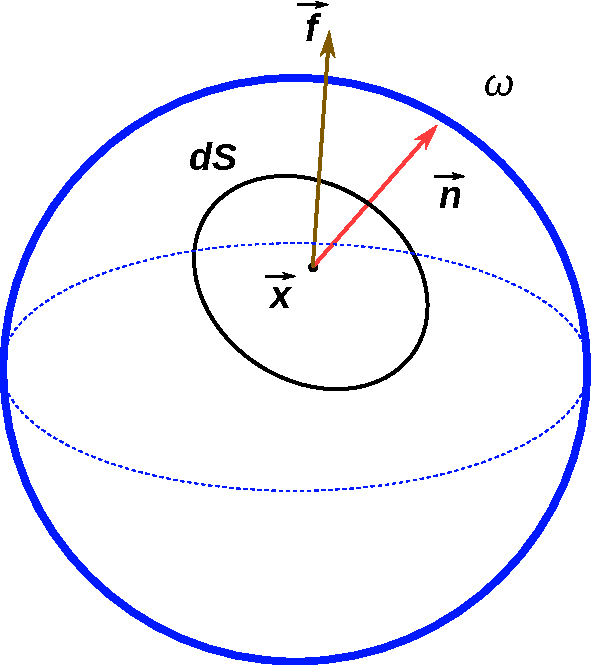
\includegraphics[width=\textwidth]{../img/sigma_def.pdf}
				
				\medskip	
				\scriptsize
				\parbox{\textwidth}{
					Выделенный объем сплошной среды $\omega$, с фиксированной точкой $\vec{x}$ внутри него и элементарной площадкой $dS$ с единичной нормалью $\vec{n}$					
				}
				
			}
		\end{column}
		\begin{column}{0.65\textwidth}
			
			\begin{exampleblock}{Замечания}
				\parbox{\textwidth}{
					\begin{itemize}[partopsep=1pt,label=\textbullet]
						\item Для определения суммарной силы, действующей на объем $\omega$, ограниченного поверхностью $S$, необходимо проинтегрировать $\vec{f}(\vec{x},\vec{n}(\vec{x}))$ по этой поверхности:
						\[
						\vec{F} = \int\limits_{S}\vec{f}(\vec{x},\vec{n}(\vec{x}))dS.
						\]
					\end{itemize}
				}
			\end{exampleblock}
		\end{column}
	\end{columns}
}





\frame{
	\frametitle{ Принцип равенства действий и противодействий  }
	
	\centering
	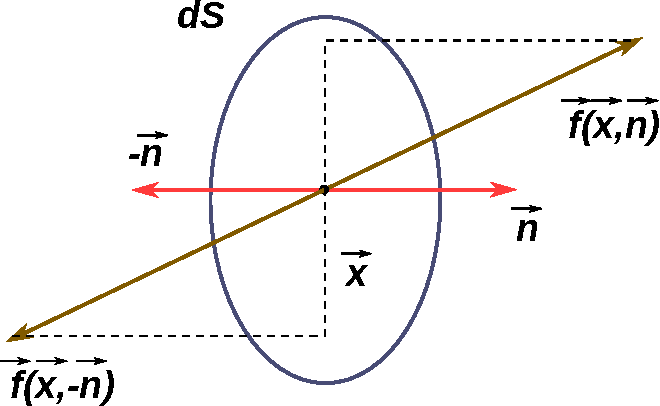
\includegraphics[width=0.5\textwidth]{../img/surface_action.pdf}\\
	{
		\scriptsize
		Иллюстрация равенства напряжения на противоположных направлениях		
	}	
	
	\bigskip
	\parbox{\textwidth}{
		Если рассмотреть напряжения, возникающие в точке $\vec{x}$ на площадке с единичной нормалью $\vec{n}$ и ей противоположной, то в следствие принципа равенства действия и противодействия
		\[
		\vec{f}(\vec{x},\vec{n}) = -\vec{f}(\vec{x},-\vec{n}).
		\]		
	}
}

\frame{
	\frametitle{ Тензор напряжений }
	
	
	\begin{columns}
		\begin{column}{0.5\textwidth}
			\centering
			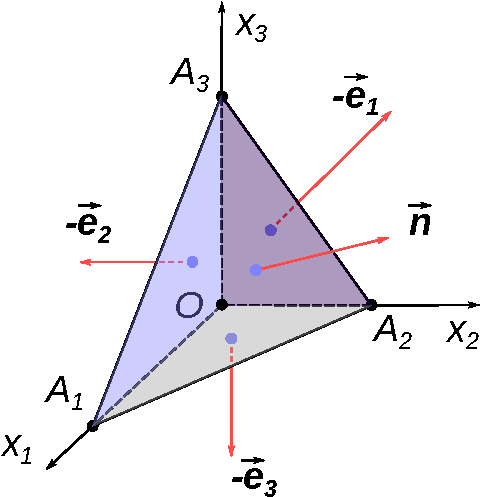
\includegraphics[width=\textwidth]{../img/cauchy_stress_tensor.pdf}
		\end{column}
		\begin{column}{0.5\textwidth}
			\parbox{\textwidth}{
			Выделим в сплошной среде, в окрестности точки $O$, тетраэдр $OA_1A_2A_3$, у которого рёбра $OA_1$, $OA_2$, $OA_3$ направлены вдоль координатных линий $x_1$, $x_2$, $x_3$, а грань $A_1A_2A_3$ перпендикулярна единичному вектору 
			\[
			\vec{n} =n_1 \vec{e}_1 + n_2 \vec{e}_2 + n_3 \vec{e}_3,
			\]
			\[
			|\vec{n}|=1.
			\]
			}
			

		\end{column}
	\end{columns}
}

\frame{
	\frametitle{ Тензор напряжений }
	
		\begin{columns}
		\begin{column}{0.4\textwidth}
			\centering
			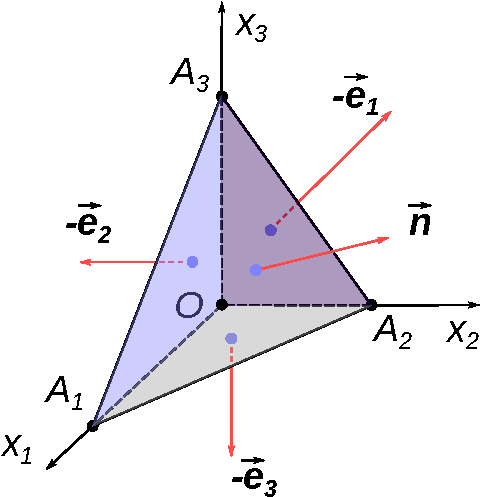
\includegraphics[width=\textwidth]{../img/cauchy_stress_tensor.pdf}
		\end{column}
		\begin{column}{0.6\textwidth}

			\begin{exampleblock}{Площади граней}
			\parbox{\textwidth}{
				\begin{eqnarray*}
				S_1 & = & S_n \cos(\vec{n},\vec{e}_1) = S_n n_1,\\
				S_2 & = & S_n \cos(\vec{n},\vec{e}_2) = S_n n_2,\\
				S_3 & = & S_n \cos(\vec{n},\vec{e}_3) = S_n n_3,
				\end{eqnarray*}
				где $S_i$, $S_n$ -- площади граней, ортогональных $\vec{e}_i$ ($i=1,2,3$) и $\vec{n}$. 
			}
			\end{exampleblock}
		
			\begin{exampleblock}{Объем тетраэдра}
				\parbox{\textwidth}{
					\[
					V = 1/3 S_n h,
					\]
					где $h$ -- длина перпендикуляра, опущенного из точки $O$ на грань $A_1A_2A_3$.
				}
			\end{exampleblock}

			
			
		\end{column}
	\end{columns}
	
}

\frame{
	\frametitle{Тензор напряжений }
	
	\begin{columns}
		\begin{column}{0.4\textwidth}
		\centering
		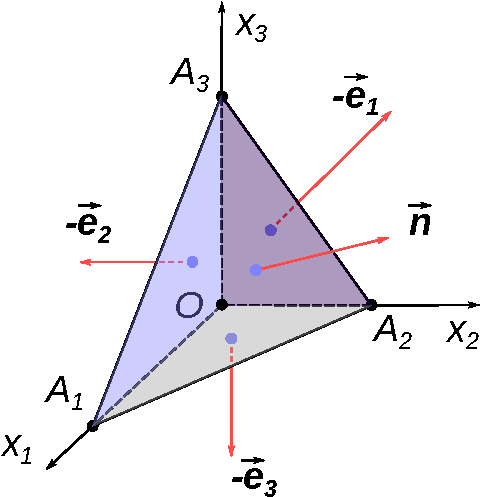
\includegraphics[width=\textwidth]{../img/cauchy_stress_tensor.pdf}
		\end{column}
		\begin{column}{0.6\textwidth}
			\begin{exampleblock}{Уравнения равновесия поверхностных сил в точке}
				\parbox{\textwidth}{
					
					\[
					\int\limits_V\vec{\Phi} dV + \int\limits_S\vec{f}(\vec{x},\vec{n}(\vec{x}))dS = 0 
					\]
					\[
					(\vec{\Phi} = \rho(\vec{F}-\vec{a})),
					\]
					где $\vec{\Phi}$ -- отнесённая к единице объёма сумма внешних объёмных сил $\vec{F}$ и сил инерции из-за ускорения $\vec{a}$ -- материальных точек.					
				}
			\end{exampleblock}
		\end{column}
	\end{columns}
	
}

\frame{
	\frametitle{ Тензор напряжений }
	
	\begin{exampleblock}{Оценка объёмного интеграла для уравнения равновесия}
		\parbox{\textwidth}{
			По теореме о среднем
			\[
			\int\limits_V\vec{\Phi} dV = \vec{\Phi}(M)V = \frac{1}{3}  \vec{\Phi}(M)S_n h ,
			\]
			где $M$ -- точка внутри тетраэдра, $V$ -- объем тетраэдра.
		}
	\end{exampleblock}
	

	
}

\frame{
	\frametitle{Тензор напряжений }
	
	\begin{exampleblock}{Разложение }
		\parbox{\textwidth}{
			Используя принцип равенства действий и противодействий имеем
			\[
			\int\limits_S\vec{f}(\vec{x},\vec{n}(\vec{x}))dS = 		\int\limits_{S_1}\vec{f}(\vec{x},-\vec{e}_1)dS +
			\int\limits_{S_2}\vec{f}(\vec{x},-\vec{e}_2)dS +		
			\int\limits_{S_3}\vec{f}(\vec{x},-\vec{e}_3)dS +
			\]
			\[			
			+\int\limits_{S_n}\vec{f}(\vec{x},\vec{n})dS =	\pause
			-\int\limits_{S_1}\vec{f}(\vec{x},\vec{e}_1)dS -
 	    	\int\limits_{S_2}\vec{f}(\vec{x},\vec{e}_2)dS -		
			\int\limits_{S_3}\vec{f}(\vec{x},\vec{e}_3)dS +
			\]
			\[
			+ \int\limits_{S_n}\vec{f}(\vec{x},\vec{n})dS =
			\]
		}
	\end{exampleblock}
	
}

\frame{
	\frametitle{ Тензор напряжения  }
	
	\begin{exampleblock}{Оценка поверхностного интеграла}
		
		\parbox{\textwidth}{
		По теореме о среднем для поверхностного интеграла  существуют точки $M_i$ и $M_n$  на поверхностях $S_i$ ($i=1,2,3$) и $S_n$, такие что
		\[
		= -S_1 \vec{f}(M_1,\vec{e}_1) -
		  S_2 \vec{f}(M_2,\vec{e}_2) -		
		  S_3 \vec{f}(M_3,\vec{e}_3) +
		  S_n\vec{f}(M_n,\vec{n}) =
		\]	\pause 
		Используя связь площадей боковых граней пирамиды тетраэдра и её основания,
		\[
			= -S_n (\vec{f}(M_1,\vec{e}_1) n_1 +
					\vec{f}(M_2,\vec{e}_2) n_2 +		
					\vec{f}(M_3,\vec{e}_3) n_3 -
					\vec{f}(M_n,\vec{n})).
		\]	
		
			
		}
	\end{exampleblock}
	
}

\frame{
	\frametitle{ Тензор напряжения }
	
	\begin{exampleblock}{Формула для напряжения на произвольной площадке}
		\parbox{\textwidth}{
			Таким образом, сокращая на $S_n$, имеем
			\[
			 -\frac{1}{3}  \vec{\Phi}(M) h =  \vec{f}(M_1,\vec{e}_1) n_1 +
			 \vec{f}(M_2,\vec{e}_2) n_2 +		
			 \vec{f}(M_3,\vec{e}_3) n_3 -
			 \vec{f}(M_n,\vec{n}).
			\]\pause
			При $h \to 0$ точки $M_i \to O$, $M_n \to O$, $M \to O$, при этом левая часть равенства стремится к $0$. \pause
			
			\medskip			
			Таким образом,  для произвольной точки $O$ \alert{
			\[
				\vec{f}(O,\vec{n}) = \vec{f}(O,\vec{e}_1) n_1 +
				\vec{f}(O,\vec{e}_2) n_2 +		
				\vec{f}(O,\vec{e}_3) n_3.
			\]}
			
		}
	\end{exampleblock}
	
}

\frame{
	\frametitle{ Тензор напряжения }
	

	
	\begin{columns}
		\begin{column}{0.45\textwidth}
			\centering
			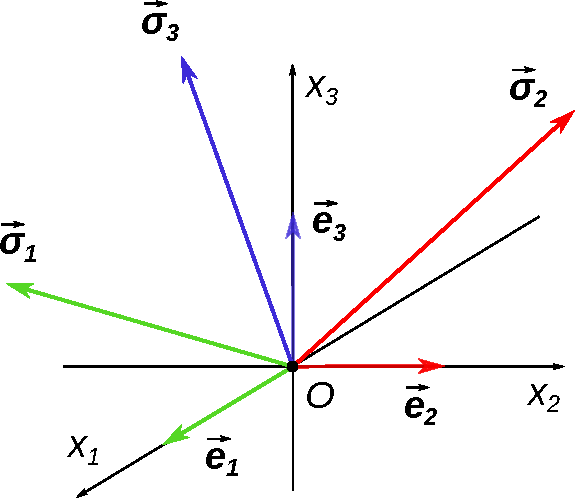
\includegraphics[width=\textwidth]{../img/sigmai_wp.pdf}
		\end{column}
		\begin{column}{0.55\textwidth}
			\parbox{\textwidth}{
				Напряжение в точке $\vec{x}$ на площадке перпендикулярной $\vec{n}$:
			\alert{
				\[
				\vec{f}(\vec{x},\vec{n}) = \vec{\sigma}_n(\vec{x}) =  n_i \vec{\sigma_i}(\vec{x})=n_i \sigma_{ij}(\vec{x})\vec{e}_j,
				\]	
				\[
				|\vec{n}|=1.
				\]
			}
			}
		\end{column}
	\end{columns}
	
	
	\begin{exampleblock}{Обозначения}
		\parbox{\textwidth}{
			\begin{eqnarray*}
				\vec{f}(\vec{x},\vec{e}_1) & = & \sigma_{11}(\vec{x})\vec{e}_1 +  \sigma_{12}(\vec{x})\vec{e}_2 +  \sigma_{13}(\vec{x})\vec{e}_3 = \vec{\sigma}_1(\vec{x}), \\
				\vec{f}(\vec{x},\vec{e}_2) & = & \sigma_{21}(\vec{x})\vec{e}_1 +  \sigma_{22}(\vec{x})\vec{e}_2 +  \sigma_{23}(\vec{x})\vec{e}_3 = \vec{\sigma}_2(\vec{x}), \\
				\vec{f}(\vec{x},\vec{e}_3) & = & \sigma_{31}(\vec{x})\vec{e}_1 +  \sigma_{32}(\vec{x})\vec{e}_2 +  \sigma_{33}(\vec{x})\vec{e}_3 = \vec{\sigma}_3(\vec{x}).
			\end{eqnarray*}
			}
		
		
	\end{exampleblock}
}

\frame{
	\frametitle{ Тензор напряжений }
	
	\begin{exampleblock}{Определение нового базиса}
		\parbox{\textwidth}{
			Рассмотрим новый базис $\vec{g}_1$, $\vec{g}_2$, $\vec{g}_3$ в заданной точке, такой что
			\[
				\vec{e}_i  = \alpha_{ij} \vec{g}_j,\quad
				\vec{g}_i  = \beta_{ij} \vec{e}_j,
			\]
			где $\alpha_{ij}$, $\beta_{jl}$ -- матрицы перехода между базисами, причём $|\alpha_{ij}|\neq 0$, $|\beta_{jl}|\neq 0$ и $\alpha_{ij}\beta_{jl}=\delta_i^l$.
		}
	\end{exampleblock}
	\begin{exampleblock}{Формулы перехода}
		\parbox{\textwidth}{
			
			\[
				\vec{n} = \bar{n}_i \vec{g}_i = \bar{n}_i \beta_{ik} \vec{e}_k= n_k \vec{e}_k.
		 	\]
			Следовательно,  $n_k = \bar{n}_i \beta_{ik}$.
			
			Тогда
			\[
				\vec{\sigma}_n = n_i \sigma_{ij}\vec{e}_j = 
				\bar{n}_k \beta_{ki}  \sigma_{ij} \beta_{jl}\vec{g}_l =
				\bar{n}_k \bar{\sigma}_{kl} \vec{g}_l,
%				
%							
%				= n_k' \alpha_{ik} \sigma_{ij}  =
			\]
			где $\bar{\sigma}_{kl} = \beta_{ki} \beta_{jl} \sigma_{ij} $.  \alert{Такое преобразование компонент матрицы $\sigma_{ij}$ является признаком смешанного тензора второго ранга.}
			
			
		}
	\end{exampleblock}	
}

\frame{
	\frametitle{Разложение напряжения}
	
	\begin{columns}
		\begin{column}{0.5\textwidth}
			\centering
			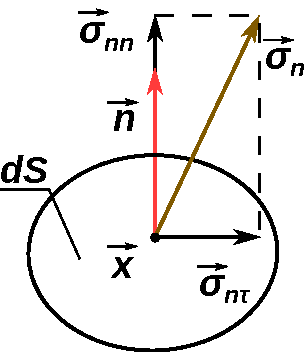
\includegraphics[width=0.7\textwidth]{../img/sigma_decomposition.pdf}
			
			\scriptsize
			Разложение напряжения на нормальную и тангенциальную составляющие
		\end{column}
		\begin{column}{0.5\textwidth}
			\parbox{\textwidth}{
				Напряжение в точке $\vec{x}$, возникающее на площадке $dS$ с единичной нормалью $\vec{n}$, можно представить в виде суммы нормальной $\vec{f}_n$ и тангенциальной составляющих $\vec{f}_\tau$:
				\[
				\vec{\sigma}_n = \vec{\sigma}_{nn}+\vec{\sigma}_{n\tau}.
				\]
				
				В этом случае $\vec{\sigma}_{nn}$ называется \alert{нормальным растяжением} или \alert{нормальным давлением}. $\vec{\sigma}_{n\tau}$ называют \alert{косым напряжением} или \alert{силой трения}.
			}
		\end{column}
	\end{columns}
	
}

\frame{
	\frametitle{ Выражения для нормальной и тангенциальной составляющих }
	\begin{columns}
	\begin{column}{0.4\textwidth}
		\centering
		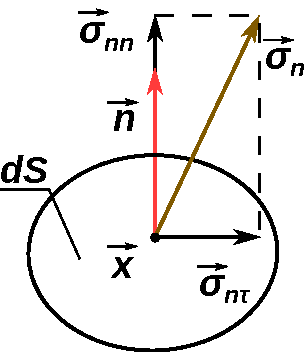
\includegraphics[width=0.7\textwidth]{../img/sigma_decomposition.pdf}
		
		\scriptsize
		Разложение напряжения на нормальную и тангенциальную составляющие
	\end{column}
	\begin{column}{0.6\textwidth}
		\begin{exampleblock}{Нормальная составляющая}
			\parbox{\textwidth}{
			\[
			\sigma_{nn} = \vec{\sigma}_n \cdot \vec{n}  = (n_i \sigma_{ij}\vec{e}_j)\cdot (n_k \vec{e}_k)=n_i n_k \sigma_{ik}.
			\]				
			}
		\end{exampleblock}\pause
		\begin{exampleblock}{Тангенциальная составляющая}
			\parbox{\textwidth}{
			\[
			\sigma_{n\tau}^2 = \sigma_n^2-\sigma_{nn}^2  = 
			\]
			\[
			=(n_i \sigma_{ij}\vec{e}_j)\cdot(n_k \sigma_{kl}\vec{e}_l)-
			n_i n_j \sigma_{ij} n_k n_l \sigma_{kl}=
			\]
			\[
			= n_i n_k \sigma_{ij} \sigma_{kl} \delta_{jl} - n_i n_j n_k n_l \sigma_{ij} \sigma_{kl}=
			\]
			\[
			=  n_i n_k \sigma_{ij} \sigma_{kl} (\delta_{jl} - n_j n_l).
			\]
			}
		\end{exampleblock}

	\end{column}
\end{columns}
}


\frame{
	\frametitle{ Главные напряжения, оси тензора напряжений }
	 
	 \begin{exampleblock}{Допущение}
	 	\parbox{\textwidth}{
	 		Будем считать, что тензор напряжений симметричный (в дальнейшем это утверждение будет обосновано)
	 		\[
	 		\sigma_{ij} = \sigma_{ji}.
	 		\]
	 	}
	 \end{exampleblock}
	 
	\begin{exampleblock}{Теорема о разложении}
		\parbox{\textwidth}{
			Для тензора напряжения в каждой точке сплошной среды существует ортонормированная система координат, в которой он имеет диагональный вид, и существуют три направления, в которых действуют только нормальные напряжения.
		}
	\end{exampleblock}
}

\frame{
	\frametitle{ Определение собственных векторов }
	
	\centering
	
	\alert{
		\Huge
		Вывод диагональности тензора в системе координат собственных векторов
	}
}



\frame{
	\frametitle{ Напряжение в системе координат главных осей}
	
	\begin{exampleblock}{}
		\parbox{\textwidth}{
		Пусть главные оси задаются ортонормированными векторами $\vec{g}_i$, а главные значения в этих осях тензора напряжения равны $\sigma_i$, тогда матрица перехода между ортонормированным базисом пространства $\vec{e}_j$ и введённым будет ортогональная (обратная совпадает с транспонированной), т.е. 
		$
		\alpha_{ij}\alpha_{kj} = \delta_{ik}.
		$
		
		\medskip
		Напряжении на площадке с нормалью $\vec{n}$ имеет вид	
		\[			
		\vec{\sigma}_n	= n_i\sigma_{ij}\vec{e}_j = \bar{n}_k \bar{\sigma}_{kl} \vec{g}_l = 
		\bar{n}_l \sigma_l \vec{g}_l,
		\]
		где $\bar{n}_k$ -- координаты нормали в базисе $\vec{g}_k$, $\bar{\sigma}_{kl} = \sigma_k \delta_{kl}$ -- тензор напряжений в главных осях.
		
		\medskip
		Таким образом, учитывая то, что $|\vec{n}|=1$, из полученной формулы видно, что  вдоль главных осей имеют место только растягивающие или сжимающие напряжения.
		}
	\end{exampleblock}
	
}
\frame{
	\frametitle{Инварианты тензора напряжений}
	
	\begin{exampleblock}{Первый инвариант}
		\parbox{\textwidth}{
			
			\[
			I_1 = \operatorname{tr} \sigma = \sigma_{11}+\sigma_{22}+\sigma_{33}=\sigma_{1}+\sigma_{2}+\sigma_{3},
			\]
			
			
		}
	\end{exampleblock}

	\begin{exampleblock}{Второй инвариант}
		\parbox{\textwidth}{
			\[
			I_2 = 
			\left|
			\begin{array}{cc}
			\sigma_{11} & \sigma_{12} \\
			\sigma_{21} & \sigma_{22}
			\end{array}
			\right|+
			\left|
			\begin{array}{cc}
			\sigma_{11} & \sigma_{13} \\
			\sigma_{31} & \sigma_{33}
			\end{array}
			\right|+
			\left|
			\begin{array}{cc}
			\sigma_{22} & \sigma_{23} \\
			\sigma_{32} & \sigma_{33}
			\end{array}
			\right| = \sigma_1\sigma_2+\sigma_2\sigma_3+\sigma_1\sigma_3,
			\]
			
		}
	\end{exampleblock}
	\begin{exampleblock}{Третий инвариант}
		\parbox{\textwidth}{
			\[
			I_3 = \operatorname{det} \sigma =
			\left|
			\begin{array}{ccc}
				\sigma_{11} & \sigma_{12} & \sigma_{13} \\
				\sigma_{21} & \sigma_{22} & \sigma_{23} \\
				\sigma_{31} & \sigma_{32} & \sigma_{33} 
			\end{array}
			\right|=
			\sigma_1\sigma_2\sigma_3.
			\]
		}
	\end{exampleblock}
	
}


\frame{
	\frametitle{ Нормальное, тангенциальное и полное напряжение в главных осях  }
	\begin{columns}
		\begin{column}{0.4\textwidth}
			\centering
			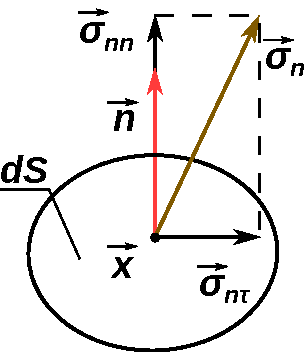
\includegraphics[width=0.7\textwidth]{../img/sigma_decomposition.pdf}
			
			\scriptsize
			Разложение напряжения на нормальную и тангенциальную составляющие
		\end{column}
		\begin{column}{0.6\textwidth}
			\begin{exampleblock}{Нормальная составляющая}
				\parbox{\textwidth}{
					\[
					\sigma_{nn} = n_i n_k \sigma_{ik} = n_i^2 \sigma_i.
					\]				
				}
			\end{exampleblock}\pause
			\begin{exampleblock}{Тангенциальная составляющая}
				\parbox{\textwidth}{
					\[
					\sigma_{n\tau}^2 = \sigma_n^2-\sigma_{nn}^2  
%					\]
%					\[
					=  n_i n_k \sigma_{ij} \sigma_{kl} (\delta_{jl} - n_j n_l)=
					\]
					\[
					= n_j n_l \sigma_j \sigma_l (\delta_{jl} - n_j n_l).
					\]
				}
			\end{exampleblock}
			\begin{exampleblock}{Полное напряжение}
			\parbox{\textwidth}{
				\[
				\vec{\sigma}_n^2 = 	(n_l \sigma_l \vec{g}_l) \cdot (n_k \sigma_k \vec{g}_k)= (n_k\sigma_k)^2.
				\]
			}
			\end{exampleblock}
			
		\end{column}
	\end{columns}
}

\frame{
	\frametitle{ Варианты напряжённого состояния }
	
	\begin{exampleblock}{Определение}
		\parbox{\textwidth}{
			Если все три главных напряжения не равны нулю, то такое напряжённое состояние называется \alert{трехосным}. Если одно из главных напряжений равно нулю, то такое напряжённое состояние называется плоским или \alert{двухосным}. Если два главных напряжения равны нулю, то такое напряжённое состояние называется \alert{одноосным}.
			
		}
	\end{exampleblock}

	\begin{exampleblock}{Давление}
		\parbox{\textwidth}{
			
			Важной характеристикой тензора напряжения является давление, определяемое первым инвариантом тензора напряжений:
			\[
			p = -\frac{1}{3}(\sigma_{11}+\sigma_{22}+\sigma_{33})=-\frac{1}{3} \sigma_{kk}.
			\]
			
			Тензор напряжения часто записывают в виде суммы шаровой и девиаторной составляющих
			\[
			\sigma_{ij} = -p\delta_{ij}+\tau_{ij}.
			\]
		
		}
	\end{exampleblock}

}

\frame{
	\frametitle{ Литература }
	\begin{itemize}
		
		\item {\em Нигматулин Р.И.} Механика сплошной среды. Кинематика. Динамика. Термодинамика. Статистическая динамика. М.:ГЭОТАР-Медиа, 2014.
	

		
	\end{itemize}
	
}


\end{document}$0$
